\chapter{De magneetzweeftrein}
\minitoc
\newpage

\section{Doelen \& structuur}
\begin{framed}
In elke practicumhandleiding vind je twee soorten doelen. De practicumdoelen vertellen wat je in het practicum gaat doen. De leerdoelen geven aan wat we willen dat je hebt geleerd na het doen van het practicum.
\end{framed}
%
\subsection{Practicumdoel}
In dit practicum bepaal je de wiskundige relatie tussen de kracht en de afstand tussen twee magneten.
%
\subsection{Leerdoel}
Na het uitvoeren van dit practicum:
%
\begin{itemize}
    \item Weet je de weg te vinden bij het natuurkundig practicum en ben je bekend met de procedure van het practicum.
    \item Ken je de basisbegrippen meetbereik, interval, herhaalbaarheid, reproduceerbaarheid en kun je deze toepassen in een onderzoek.
    \item Kun je meetfouten en meetonzekerheden door rekenen. 
    \item Kun je data analyseren en presenteren m.b.v. Python.
    \item Ken je de basisprincipes en onderdelen van een verslag in het algemeen en specifiek resultaten, discussie en conclusie.
\end{itemize}
%
\subsection{Structuur}
IE-1 bestaat uit verschillende deken:
%
\begin{itemize}
    \item Voorbereiding \& Uitvoering 
    \item Analyseren van de data
    \item Verslagmiddag 1
    \item Geven en ontvangen van feedback
    \item Verslagmiddag 2
\end{itemize}
%
Het verslag maak je met de partner waarmee je samenwerkt.
%
\section{Inleiding}
Magneetzweeftreinen blijven vlak boven de grond zweven doordat ze gebruik maken van magneten die elkaar afstoten en aantrekken. In het ontwerpen van de magneetzweeftrein is het modelleren van het gedrag van de trein bij hoge snelheden van groot belang. Zonder een goed computermodel zal het niet mogelijk zijn om een goed werkend prototype te maken. \newline\newline
%
Een van de factoren die van invloed is op het gedrag van de trein is de afstand tussen de grond en de trein en de demping wanneer er over een niet volledig horizontaal traject wordt gereden. Om dat te kunnen modelleren is het van belang dat de precieze relatie tussen de afstand tussen de magneten en de grootte van de afstotende kracht bekend is. Alhoewel de theorie een goede indruk geeft van deze relatie, zal deze relatie voor niet ge\"{i}dealiseerde situaties experimenteel bevestigd moeten worden. Het is belangrijk om inzicht te krijgen in hoeverre de ge\"{i}dealiseerde theorie in staat is de praktijk te benaderen (of vice versa). De onderzoeksvraag wordt daarmee:
\newline
\begin{center}
\textit{Hoe hangt de kracht tussen twee tegenover elkaar geplaatste schijfmagneten af van de afstand tussen de magneten?}
\end{center}

\begin{framed}De hoofdonderzoeker die het onderzoek zou uitvoeren is in het buitenland en kan onmogelijk het onderzoek afronden. Jij en je partner zijn aangesteld als de vervanger van de hoofdonderzoeker en moeten een overtuigend antwoord op deze onderzoeksvraag geven. Gelukkig ligt er een theoretische afleiding voor een natuurkundig model en zijn er door de hoofdonderzoeker een introductie en methode geschreven. Deze staan hieronder uitgewerkt. De methode is goed genoeg beschreven om de daadwerkelijke metingen uit te voeren. Helaas zijn wel alle meetonzekerheden en de daarbij behorende berekeningen niet uitgevoerd. Ook die berekeningen en afleidingen moeten door jullie gemaakt worden.
\end{framed}

\newpage
\begin{center}
    \LARGE{Uit het rapport van de onderzoeker}
\end{center}

\section{Theoretische achtergrond}
\subsection{Schijfmagneten}
In dit experiment wordt gebruik gemaakt van twee schijfmagneetjes. Een schijfmagneetje is een kleine magneet in de vorm een platte cilinder, zie figuur \ref{fig:magneten}. De permanente schijfmagneetjes van deze proef zijn gemaakt van de ferromagnetische verbinding Nd$_2$Fe$_{14}$B. Het symbool Nd staat voor het zeldzame aardmetaal neodynium. Fe staat voor het element ijzer, terwijl het symbool B het element boor aanduidt. Nd$_2$Fe$_{14}$B magneten zijn de sterkste commercieel verkrijgbare magneten en worden toegepast in o.a. motoren, luidsprekers en magnetische lageringen. Zelfs bij de kleine afmetingen als gebruikt in deze proef zijn Nd$_2$Fe$_{14}$B magneten zeer krachtig.
%
\begin{figure}[h!]
    \centering
    \includegraphics[width=0.3\linewidth]{Figures/IE1/magneten.eps}
    \caption{Krachten tussen schijfmagneetjes in geval van aantrekking. $F_{21}$  is de kracht die magneet 2 uitoefent op magneet 1 en $F_{12}$ is de kracht die magneet 1 uitoefent op magneet 2. De twee afstanden tussen de magneetjes zijn aangeduid.}
    \label{fig:magneten}
\end{figure}
%
\subsection{Magnetische dipolen}
Eigenschappen van het magnetisch veld van een schijfmagneet kunnen grotendeels afgeleid worden uit de benadering dat een schijfmagneet opgevat mag worden als een klassieke magnetische dipool. Een klassieke magnetische dipool is een kleine draadlus waardoorheen een elektrische stroom loopt. Figuur \ref{fig:magneetvelden}a geeft een voor\-stelling van zo\textquotesingle n dipool met het bijbehorend patroon van magnetische veldlijnen. De dipool wordt gekarakteriseerd door het magnetisch dipoolmoment \(\vec{m}=I\vec{A}\) , een vector (met grootte en richting). Hierin is:
%
\begin{itemize}
    \item $I$ de grootte van de stroom door de lus in A
	\item $A$ het oppervlak van de lus in m$^2$
	\item $m$ het magnetische dipoolmoment in Am$^2$
\end{itemize}
%
Het oppervlak is hier een vector waarvan de richting bepaald wordt door de richting van de stroom en gevonden kan worden met behulp van de rechterhandregel. Een puntdipool ontstaat in de limiet waarbij het oppervlak van de lus naar nul gaat en de stroom naar oneindig, zodanig dat het product \(\vec{m}=I\vec{A}\), constant blijft.
%
\begin{figure}[h!]
    \centering
    \includegraphics[width=0.8\linewidth]{Figures/IE1/magneetvelden.eps}
    \caption{Klassieke magnetische dipool (a), gevormd door een stroomvoerende draadlus, met het bijbehorend patroon van magnetische veldlijnen. Ferromagetische dipool (b), opgebouwd uit een N-pool en een Z-pool, eveneens met veldlijnenpatroon. Naar \cite{grant_electromagnetism_2008}, na aanpassing}
    \label{fig:magneetvelden}
\end{figure}
%
Kleine ferromagneten zoals de magneetschijven in dit experiment zijn ook magnetische dipolen, die je opgebouwd kan denken uit een noordpool (N-pool) en een even sterke zuidpool (Z-pool) met een kleine tussenafstand tussen de polen. In Figuur \ref{fig:magneetvelden}b is een magnetische dipool met het veldlijnenpatroon afgebeeld. Het magnetisch veld van de klassieke en ferromagnetische dipool hebben hetzelfde ruimtelijke patroon. Als een ferromagneet maar klein genoeg is, kan deze ook gezien worden als een puntdipool.  Omgekeerd, gezien van grote afstand, gedraagt iedere magnetische dipool (bijvoorbeeld de aarde) zich als een magnetische puntdipool. 
%
\subsection{De kracht tussen magnetische dipolen}
Twee magneten oefenen niet alleen een aantrekkende of afstotende kracht op elkaar uit, maar ook een moment: ze ori\"{e}nteren zich in elkaars veld. Het richten van een kompasnaald in het aardmagnetisch veld is een bekend voorbeeld van dit effect.\\

In dit experiment concentreren we ons alleen op de kracht tussen magneten. Om daarvoor een formule te vinden, starten we vanaf de wisselwerkingsenergie $U$ van twee magnetische puntdipolen \(\vec{m_1}\) en \(\vec{m_2}\) op onderlinge afstand \(\vec{r}\). Dat is de potenti\"{e}le energie van één van de dipolen in het magnetisch veld van de andere. Zonder afleiding presenteren we hier de formule voor $U$:
%
\begin{equation}\label{eq:potfieldB}
    U=\frac{\mu}{4\pi}\left(\frac{\vec{m_1}\cdot\vec{m_2}}{r^3}-\frac{3(\vec{m_1}\cdot\vec{r})(\vec{m_2}\cdot\vec{r})}{r^5}\right )
\end{equation}
%
Hierin is $\mu$ is de permeabiliteit van het medium en \(\vec{r}\) de vector die dipool 1 verbindt met dipool 2. Voor lucht als medium mag $\mu_0$ genomen worden, de permeabiliteit van het vacuüm. De producten in formule \ref{eq:potfieldB} met een punt ($\cdot$) zijn zogenoemde inwendige
producten (pro memorie: \(\vec{a}\cdot\vec{b}=\abs{\vec{a}}\abs{\vec{b}}\cos(\theta)\) met $\theta$ de hoek tussen de vectoren \(\vec{a}\) en \(\vec{b}\) ). Als geldt  \(\vec{m_1}=\vec{m_2}=m\) en als de dipoolmomenten antiparallel of parallel langs de verbindingsvector \(\vec{r}\) liggen, reduceert formule \ref{eq:potfieldB} voor lucht als medium tot:
%
\begin{equation}\label{eq:potentialfield}
     U=\pm \frac{\mu_o}{2\pi}\frac{m^2}{z^3}
\end{equation}
%
De energie is positief als de dipolen antiparallel zijn (afstoting) en negatief als deze parallel zijn (aantrekking). In formule \ref{eq:potentialfield} is de afstand $r$ vervangen door de verticaal veronderstelde afstand $z$ (als in het experiment). Aangezien de kracht de plaats afgeleide is van de potentiele energie, geldt er voor de magnetische kracht tussen de dipolen (we negeren hier de richting van de kracht en defini\"{e}ren impliciet de constante $\alpha$):
%
\begin{equation} \label{eq:model}
    F_m(z) = \frac{dU}{dz} = \frac{3\mu_0m^2}{2\pi}\frac{1}{z^4}=\frac{\alpha}{z^4}
\end{equation}
%
Vaak wordt ter karakterisering van een permanente magneet het remanente veld $B_r$ gebruikt \citep{supermagnete_data_sheet_s-10-05-npdf_2011}. Dat is het magnetisch veld van de magneet dat permanent overblijft of achterblijft na magnetisatie. Het remanente veld wordt geven door:
%
\begin{equation}\label{eq:Br}
    B_r = \mu_0 \frac{m}{V}
\end{equation}
%
In formule \ref{eq:Br} is $V$ het volume van de magneet, zodat het remanente veld gezien kan worden als een dipool\-dichtheid.\\

De hier gepresenteerde theorie is van toepassing op puntdipolen. De schijfmagneetjes van deze proef zijn echter geen punten, maar hebben een zekere ruimtelijke uitgebreidheid. Daarom kan in het experiment mogelijk een afwijking gevonden worden van de afstandsafhankelijkheid als beschreven door formule \ref{eq:model}.
%
\section{Introductie}
Voor het ontwerpen van nieuwe, snellere en veiligere zweeftreinen is het essentieel om accurate computermodellen te gebruiken die het rijgedrag van de zweeftrein kunnen simuleren. Voor een accuraat computermodel is een model van de relatie tussen de afstand tussen de twee magneten en de onderlinge kracht essentieel \citep{sanagawa2001characteristics}. In dit onderzoek wordt een model dat gebaseerd is op de superpositie van magnetische puntdipolen getest. 
\newline
Het model, afgeleid en beschreven in \cite{Pols}, gaat ervan uit dat de totale potentiele energie van de magneten gelijk is aan de som van potentiele energie van magnetische puntdipolen. Met het gegeven dat de kracht gelijk is aan de afgeleide van de potentiele energie naar de afstand, geldt voor de kracht tussen twee magneten:
%
\begin{equation}
F_{m}(z)=\frac{3 \mu_{0} m^{2}}{2 \pi} \frac{1}{z^{4}}=\alpha \frac{1}{z^{4}}
\end{equation}
%
Hierin is $\mu_0$ de magnetische permeabiliteit, $m$ het magnetische dipoolmoment en $z$ de hart-tot-hart afstand van de twee magneten. Dit model wordt gevalideerd aan de hand van een experimentele opzet waarbij de afstotende en aantrekkende kracht tussen twee magneten en hun onderlinge afstand wordt bepaald. Uit het experiment wordt het remanente veld bepaald:
%
\begin{equation}
B_{r}=\mu_{0} \frac{m}{V}
\end{equation}
%
Het model is gevalideerd wanneer de experimentele waarden het verwachtte vierde machtsverband gedrag vertonen en het remanente veld volgend uit de empirische data overeenkomt met de specificaties van de magneten. Daartoe richten we ons op de volgende twee onderzoeksvragen:
%
\begin{enumerate}
    \item \textit{Hoe hangt de afstotende/aantrekkende kracht tussen twee magneten af van hun onderlinge afstand?}
    \item \textit{Is het theoretische model van een superpositie van dipolen voldoende om die relatie te beschrijven?}
\end{enumerate}{}
%
Dit onderzoek is uitgevoerd als onderdeel van het vak Natuurkundig Practicum aan de TU Delft.
%
\section{Experimentele methode}
\subsection{Experiment en instrumentatie}
Voor het valideren van het voorgestelde model wordt gebruik gemaakt van een opstelling waarbij twee magneten boven elkaar hangen en de onderlinge kracht bepaald wordt, zie figuur \ref{fig:IE1opstelling}. De hart-tot-hart afstand (figuur \ref{fig:IE1opst_onz}) tussen de twee magneten wordt gegeven door:
%
\begin{equation}
z=\frac{1}{2} d_{m}+h_{1}+h_{1,2}+h_{2}+\frac{1}{2} d_{m}
\label{eq:afstanden}
\end{equation}
%
Voor bepaling van $h_1$ en $h_2$ wordt een schuifmaat \href{https://youtu.be/eBG2Y0nXGAs}{\faCamera} gebruikt met een meetonzekerheid van ... mm, $h_{1,2}$ wordt bepaald m.b.v. een liniaal met een meetonzekerheid van ... mm. Volgens de specificatie van de magneet is de meetonzekerheid in de diameter van de magneet ... mm \citep{supermagnete_data_sheet_s-10-05-npdf_2011}. Dit levert een totaal meetonzekerheid van $u(r)$= ... mm. Zie de Appendix voor de bijbehorende afleiding.

\begin{figure}[h!]
    \centering
    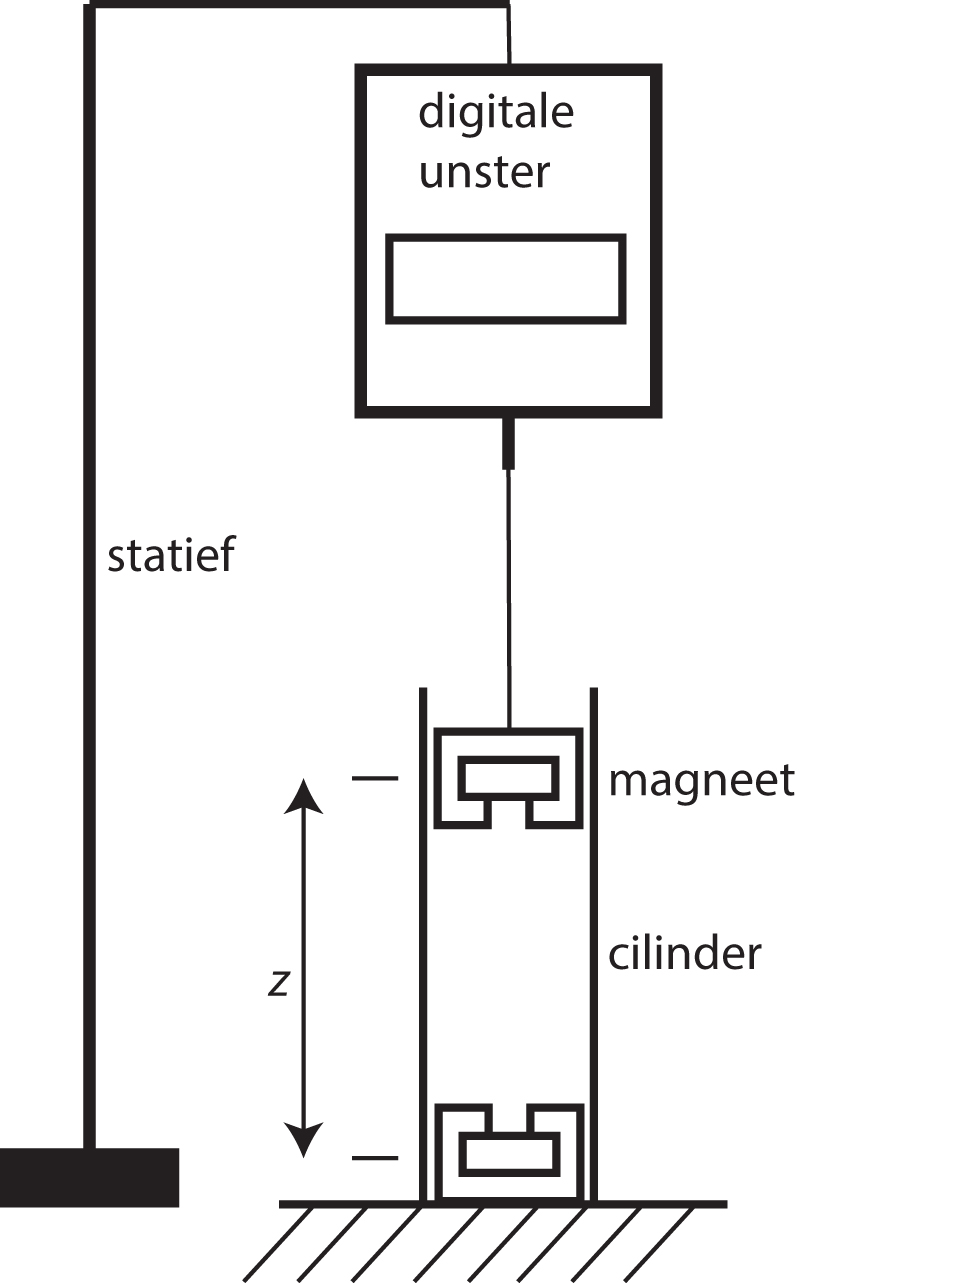
\includegraphics[width=0.35\linewidth]{Figures/IE1/opstelling.eps}
    \caption{De opstelling waarbij de bovenste magneet gepositioneerd wordt t.o.v. de gefixeerde magneet. De onderlinge kracht wordt bepaald m.b.v. een digitale unster.}
    \label{fig:IE1opstelling}
\end{figure}

Met behulp van een digitale unster (Christen Orange OR-42) met een afleesnauwkeurigheid van ... g wordt de onderlinge uitgeoefende kracht bepaald:
%
\begin{equation}\label{eq:Fz}
F_{1,2}=\Delta m \cdot g
\end{equation}
%
hierin is $g$ de zwaartekrachtsversnelling in Nederland met een waarde van \SI{9.812\pm 0.001}{m\per s^2} en $\Delta$m het verschil in massa in kg gegeven door:
%
\begin{equation}
\Delta m=m_{\infty}-m_{r}
\end{equation}
%
Hier is $m_{\infty}$ de massa op ‘oneindige’ afstand van de vaste magneet en $m_r$ de gemeten massa op afstand $r$ van de vaste magneet.
Aangezien de meetonzekerheid in $g$ velen malen kleiner is dan de meetonzekerheid in $m$, geldt 
$u(F) = \SI{1e-2}{N}$, zie de appendix voor de afleiding.

\subsection{Procedure}
In de eerste meetserie wordt gebruik gemaakt van twee aantrekkende magneten. De bovenste magneet wordt langzaam naar de onderste magneet bewogen. Het punt waarbij de eerste uitwijking van de unster ($\Delta m \ne 0$) en de grootst mogelijke kracht tussen de magneten wordt bepaald. Vervolgens worden de daadwerkelijke metingen uitgevoerd met een krachtsinterval van grofweg $\frac{F_{max}-F_{min}}{10}$. Deze keuze voor interval zorgt er voor dat met name op korte afstanden, overeenkomstig met de afstand tussen de magneten van treinen, veel metingen gedaan worden. Bovenstaande procedure wordt herhaald voor een verzwaarde afstotende magneet. 
%
\begin{figure}[h!]
    \centering
    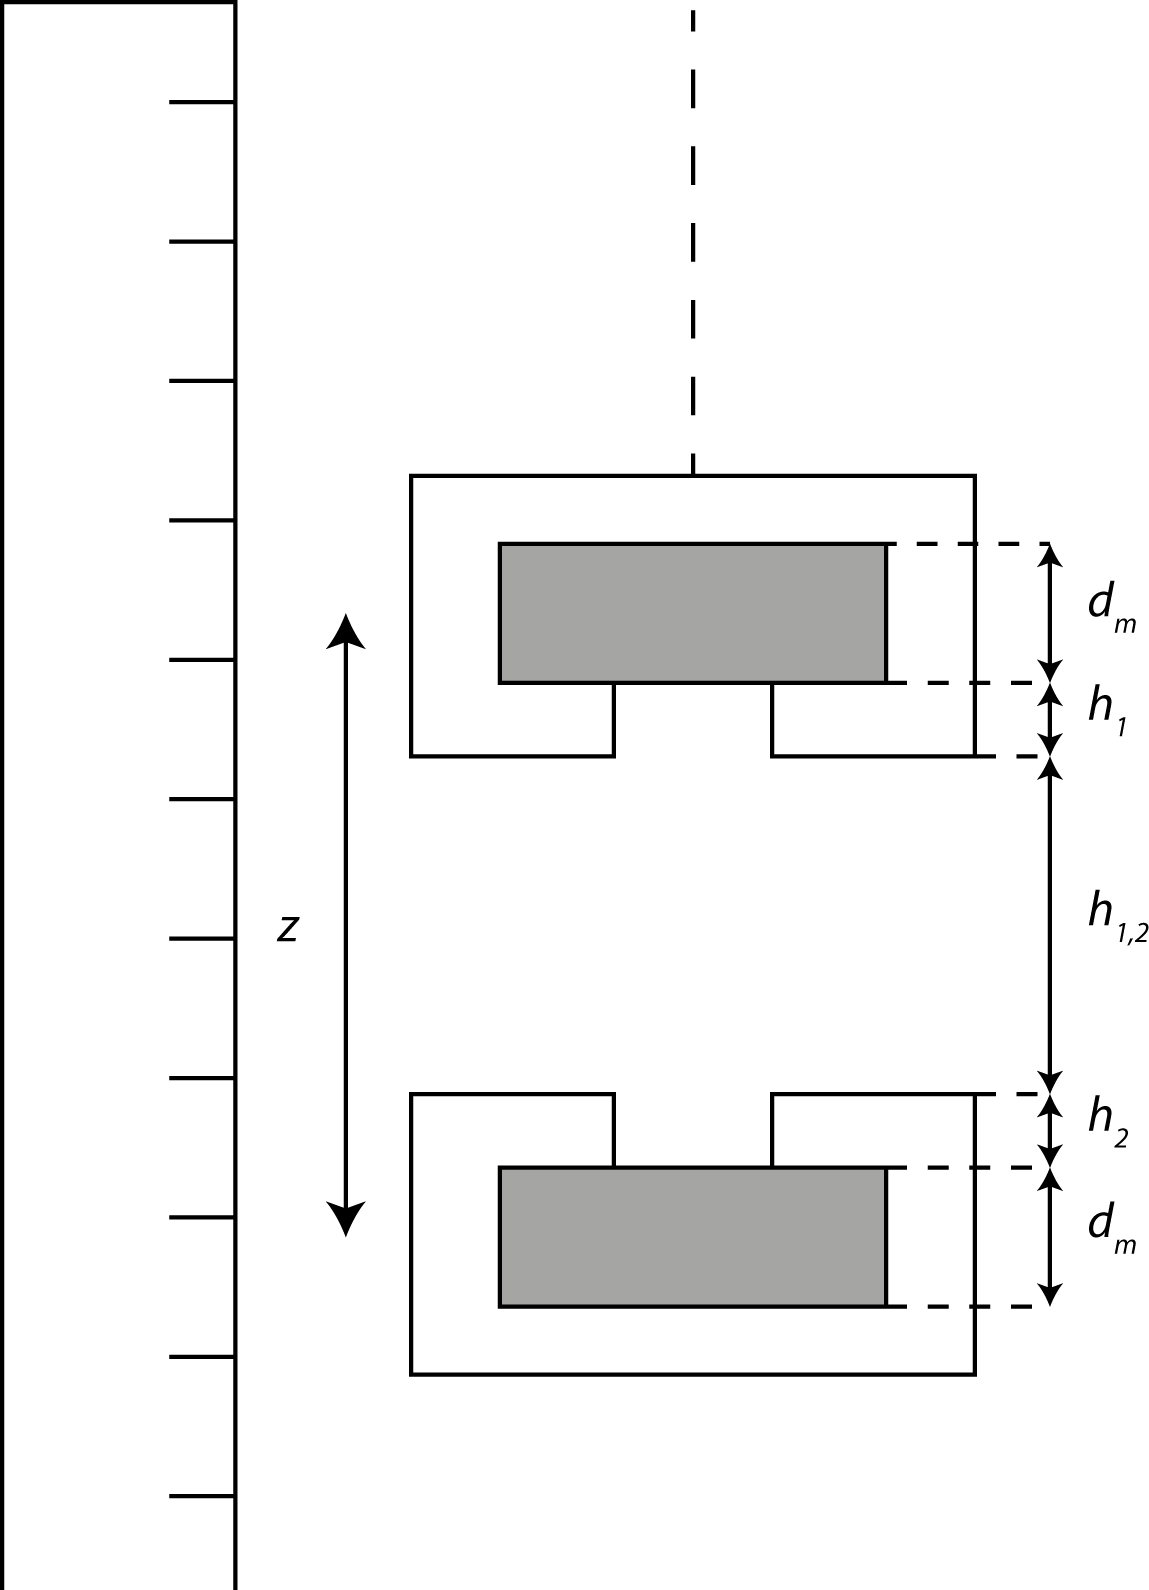
\includegraphics[width=0.3\textwidth]{Figures/IE1/ie1_opst_onz.eps}
    \caption{De close up van de twee magneten (grijs) in hun plastic omhulsel laat de verschillende te bepalen grootheden zien, waarbij de hart-tot-hart afstand gegeven wordt door formule \ref{eq:afstanden}}.
    \label{fig:IE1opst_onz}
\end{figure}

\begin{center}
    \LARGE{Einde rapport van de onderzoeker}
\end{center}

\bibliographystyle{dcu}
\bibliography{Chapters/part3/IE1.bib}
\newpage
%
\section{Opdrachten practicummiddag}
Voer de volgende opdrachten uit:
\begin{itemize}
    \item Meet alle afstanden uit Vergelijking \ref{eq:afstanden} behalve $h_{1,2}$.
    \item Doe de afleiding voor de onzekerheid in de afstand en de kracht. Deze zouden beschreven staan in de Appendix, maar de Appendix is niet terug te vinden in de documenten van de hoofdonderzoeker.
    \item Volg de beschreven meetprocedure. Voer de definitieve metingen uit voor de relatie tussen kracht en afstand. Noteer de uitkomsten in de excel (zie Brightspace). Noteer de meetonzekerheden in het Jupyter Notebook (labjournaal).
    \item Verwerk alle metingen in de Jupyter Notebook (te vinden op Brightspace).
    \item Maak de eerste plot.
    \item Laat je plot controleren door de TA.
\end{itemize}
%
\newpage
\newpage
\section{Opdrachten data-analyse}
Je hebt je data verzameld en een eerste plot gemaakt. Nu ga je de data analyseren door :
%
\begin{itemize}
    \item Een errorbarplot te maken met curve fit. 
    \item Te onderzoeken of er eventueel sprake is van een systematische fout en daarvoor compenseren.
    \item Het vierde machtsverband onderzoeken met behulp van een linearizatie.
    \item Het remanente veld berekenen en vergelijken met het remanente veld gemeld in de specificaties.
\end{itemize}
Om je te helpen bij deze analyse, staan de stappen ook vermeld in het notebook.
%
\section{Verslagmiddag 1\&2}
\subsection{Voorbereiding}
Om de twee eerste verslagmiddagen effectief en effici\"{e}nt te besteden is een goede voorbereiding noodzakelijk. Lees daarom vooraf:
\begin{itemize}
    \item Het hoofdstuk over schrijven in dit dictaat
    \item Whitesides’ Group: Writing a Paper
    \item Unspoken rules for writing a paper
    \item Robert Pirsig' on the scientific method
\end{itemize}
Deze documenten zijn te vinden de appendix.
%
\subsection{Introductie tot verslaglegging}
Je hebt een experiment gedaan waarbij je alles wat nodig is om het experiment te begrijpen en de conclusies na te gaan in je labjournaal / logboek hebt gezet. Waarom dan toch nog een verslag of artikel schrijven over dat experiment? 
Een belangrijke reden van schrijven is het structureren van je eigen gedachten: Wat heb je nu precies gedaan in dit experiment? Wat leer je daarvan? Wat zijn mogelijkheden tot vervolgonderzoek? Waar kan het beter? Door het schrijven van het verslag begrijp je nog beter wat er is gedaan, waarom dat is gedaan en wat de relevantie daarvan is. Schrijven = begrijpen.\newline\newline
%
Een tweede belangrijke reden voor het schrijven van het verslag is het delen van kennis. Wanneer je aan de rand van onze wetenschappelijk kennis zit, betekent het delen van die kennis vooruitgang. Je helpt jezelf maar ook anderen om te komen tot nieuwe kennis (het delen van die nieuwe kennis is in de wetenschap ook vaak een manier om geld voor (nieuw) onderzoek te krijgen).\newline\newline 
%
Een derde belangrijke reden voor het schrijven van het verslag is de controle op de kennis die is ontwikkeld. In de wetenschap wordt dat gedaan aan de hand van peer review. Dit is een check of wat er geclaimd wordt daadwerkelijk ondersteund wordt door de data. Dit betekent dat de betrouwbaarheid van de data en de validiteit van de conclusies onderzocht worden door andere experts.\newline\newline 
%
De drie voor TN meest relevante functies van verslaglegging kunnen als volgt worden samengevat: \textit{De functie van een wetenschappelijk verslag is jezelf en anderen ervan overtuigen dat wat er is gedaan het best mogelijk antwoord geeft op de gestelde onderzoeksvraag.} 
%
\subsection{Argumentatie}
Om anderen te overtuigen gebruik je argumentatie: Een onderbouwing voor wat er gedaan is en wat daaruit komt. Toulmin [1] levert daartoe een goede argumentatiestructuur, zie figuur \ref{fig:Toulmin}. In dat model wordt er een link gelegd tussen de te maken claim (de conclusie) en de data. 

\begin{figure}
    \centering
    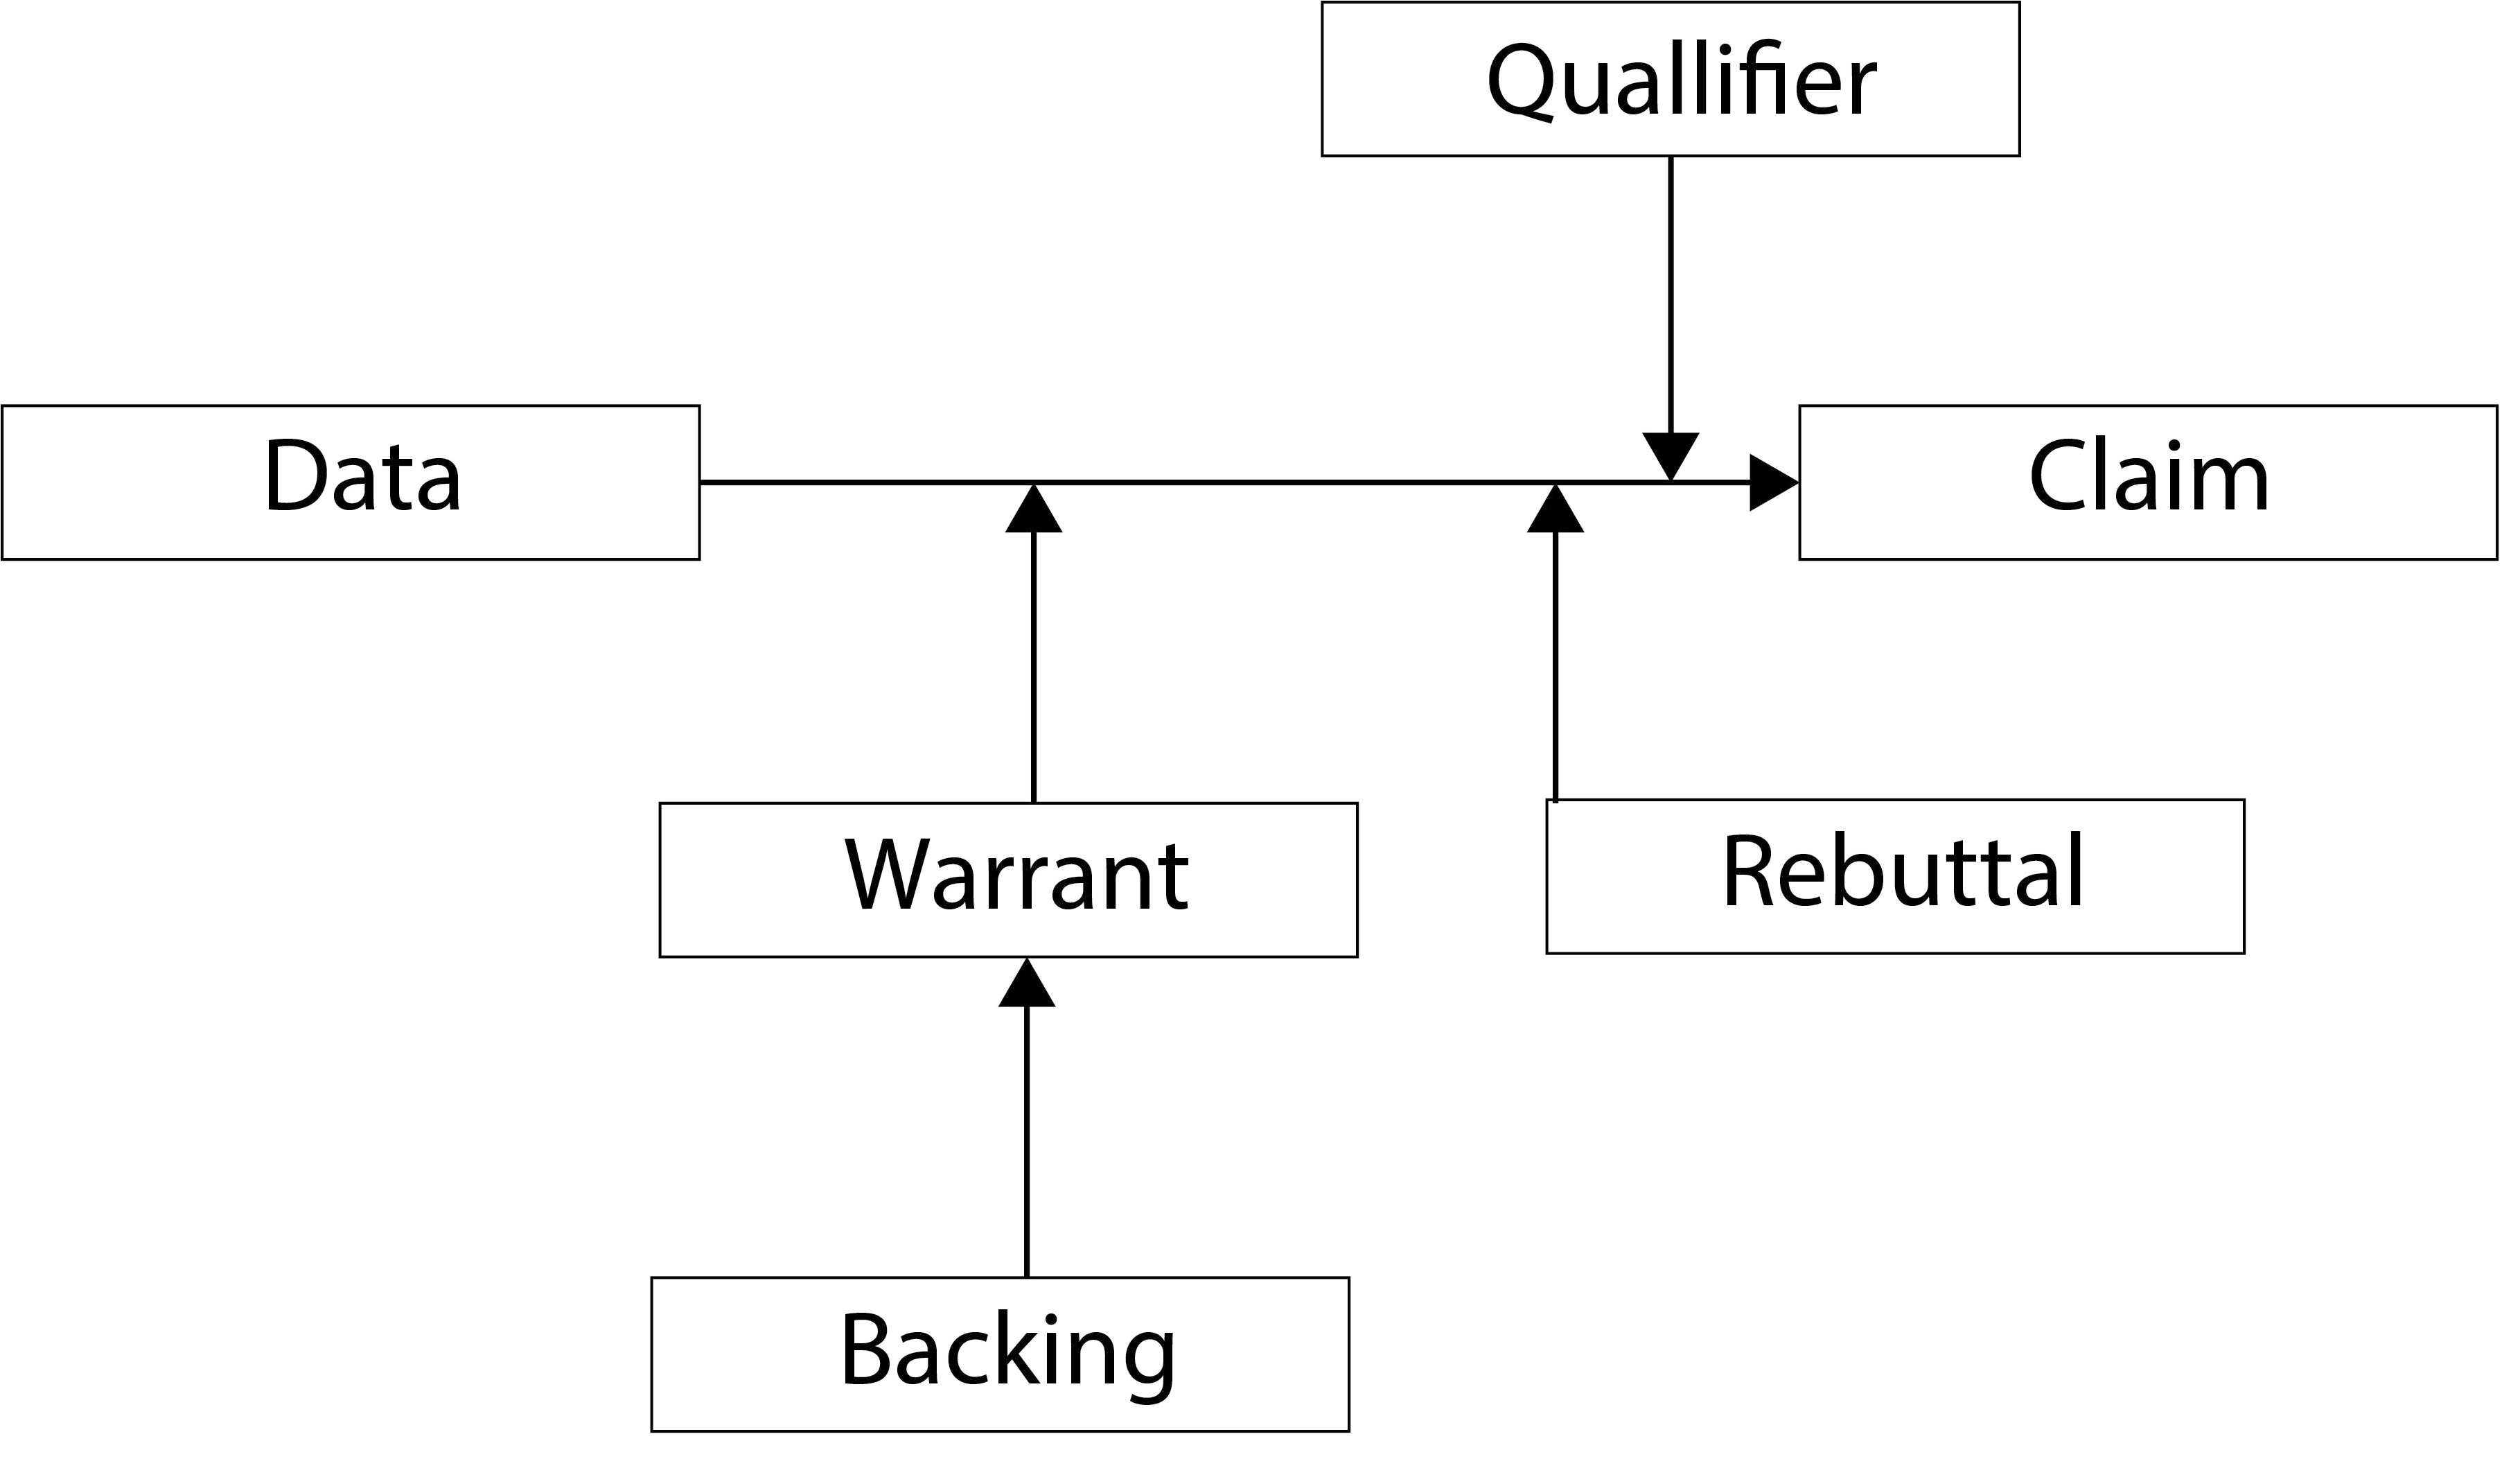
\includegraphics[width=0.5\textwidth]{Figures/general/Toulmin.eps}
    \caption{Het Toulmin (2003) argumentatie model legt een verbinding tussen de te maken claim en de primaire data.}
    \label{fig:Toulmin}
\end{figure}

Het model van Toulmin bestaat uit de volgende elementen:
\begin{itemize}
    \item Claims: De conclusies die gemaakt worden.
    \item Data: De data die gebruikt zijn als bewijs voor de claim.
    \item Warrants: De onderbouwing die de link tussen data en claim rechtvaardigt.
    \item Backing: De onderliggende onderbouwing, vaak de natuurkundige en wiskundige 	theorie\"{e}n die ten grondslag liggen.
    \item Qualifiers: De condities waaronder de claim geldig is (validiteit van de conclusie).
    \item Rebuttals: Tegenwerpingen voor de claim (de claim is niet geldig als).
\end{itemize}
%
Niet alle elementen worden expliciet genoemd in een verslag of artikel, maar zijn vaak wel terug te vinden. Zo zijn qualifiers te vinden in de methodesectie waarin beschreven wordt wat er gedaan is (\textit{in dit experiment is er sprake van supergeleiding voor T $<$ 50 K}). Belangrijk voor het schrijven van een natuurkundig verslag zijn de warrants: Wat is de onderbouwing die je claims rechtvaardigt (\textit{uit de vergelijking van de verwachte fitlijn met de experimentele data en het vergelijken van het berekende remanente veld met de literatuurwaarde volgt dat ...}). 
%
\subsection{Structuur van een verslag}
Om anderen ervan te overtuigen dat jouw antwoord op de onderzoeksvraag het best mogelijke antwoord is, gegeven de condities (tijd, geld, kennis), en dat beantwoording van die vraag ook relevant is, wordt er een meestal een vaste structuur gehanteerd voor een verslag. Die structuur, en de functie van de onderdelen, staan samengevat in tabel \ref{tab:structuurverslag}. Alhoewel dit de meest voorkomende structuur is voor het maken van een verslag of artikel, zijn andere structuren ook mogelijk en stellen verschillende journals andere eisen [2].
%
\begin{table}[H]
    \centering
    \caption{De belangrijkste onderdelen en hun bijbehorende functies van een wetenschappelijk verslag.}
    \begin{tabular}{l|l}
         \textbf{Onderdeel} & \textbf{Functie/vraag} \\
         \hline
         Samenvatting &	Korte beschrijving van wat, waarom en uitkomst.\\
         Inleiding	& Wat is er gedaan / wat is de aanleiding?\\
         Experimentele methode &	Hoe gedaan, wat is speciaal?\\
         Resultaten	& Wat is er gevonden?\\
         Discussie & Wat “betekenen” de resultaten?\\
         Conclusie & Wat is het antwoord op de onderzoeksvraag?\\
         Referenties & Welke bronnen zijn gebruikt?\\
    \end{tabular}
    \label{tab:structuurverslag}
\end{table}
%
\textbf{Samenvatting:} Geeft een korte beschouwing van wat er is gedaan, waarom en hoe. De belangrijkste resultaten en conclusies worden gepresenteerd. Normaal gesproken wordt er een woordlimiet van ongeveer 250 aangehouden.\newline\newline
%
\textbf{Inleiding:} Sets the scene. Vanuit een breed perspectief wordt er gewerkt naar de specifieke onderzoeksvraag. In de introductie wordt ook een kort overzicht gegeven van wat er reeds gedaan is. Duidelijk moet worden wat er in dit onderzoek gedaan wordt en waarom.\newline\newline
%
\textbf{Experimentele methode:} Hierin wordt duidelijk gemaakt wat het experiment precies inhoudt, en wat de te volgen procedure is. Een goede beschrijving maakt het mogelijk om het experiment te reproduceren en om biedt de mogelijkheid voor andere experts om na te gaan of het experiment daadwerkelijk antwoord kan geven op de onderzoeksvraag.\newline\newline
%
\textbf{Resultaten:} In deze sectie presenteer je de data die de uiteindelijke claim ondersteunen. Denk hierbij goed na over welke data en in welke vorm je deze wilt presenteren. Daarbij is het belangrijk dat je je keuze verantwoordt.\newline\newline
%
\textbf{Discussie:} In de discussie interpreteer je de data en relateer je deze met eerder werk. Voor kleinere onderzoeken is een aparte discussie sectie niet nodig. Discussie en resultaten worden dan samengenomen.\newline\newline
%
\textbf{Conclusie:} In de conclusie geef je antwoord op de onderzoeksvra(a)g(en). Daarbij komt voor de lezer eigenlijk geen nieuwe informatie. De conclusie geeft een kernachtig verslag van wat er is gevonden. Je geeft hier het belangrijkste discussiepunt en mogelijkheden voor vervolgonderzoek.\newline\newline
%
\textbf{Referenties:} Hierin staan alle bronnen die gebruikt zijn en waarnaar je refereert in de tekst. Er zijn diverse programma’s die je helpen, waaronder EndNote voor Word en voor LaTeX. Deze software pakketten maken het goed mogelijk om de uiteindelijke opmaak van de referenties (bijv APA-style) automatisch te laten uitvoeren.\newline\newline
%
\subsection{Layout}
Een van de belangrijkste regels voor de layout is dat het geheel overzichtelijk is, dat de structuur helder is. Maak voor de verslagen gebruik van de template die je krijgt op de LaTeX middag. 
%
\subsection{Vragen}
Voor het verslag van IE-1 is de introductie en experimentele methode geschreven. De resultaten en conclusie moet je zelf nog schrijven. De onderstaande vragen helpen je daarbij. Beantwoord de vragen (dit mag digitaal).\newline\newline
%
\textbf{Introductie:}
\begin{enumerate}
    \item Wat doet de onderzoeker in de eerste zin van de introductie? En in de eerste alinea?
    \item Waarom worden de formules genummerd?
    \item Hoe zijn de twee onderzoeksvragen complementair aan elkaar?
\end{enumerate}
%
\textbf{Experimentele methode:}
\begin{enumerate}
    \item Hoe wordt in de eerste zin de introductie gekoppeld met de experi\-mentele methode?
    \item Is in de eerste paragraaf (experiment en instrumentatie) duidelijk wat de te volgen procedure is? Zo nee, wat is dan de functie van deze paragraaf?
    \item Leg uit wat je vindt van de twee gebruikte figuren. Zijn beide figuren nodig?
\end{enumerate}
%
\textbf{Resultaten (en discussie)}
Bekijk de verschillende grafieken die je hebt gemaakt en beantwoord de volgende vragen:
\begin{enumerate}
    \item Welke wil je gaan gebruiken voor het verslag?
    \item Waarom kies je specifiek voor deze grafiek(en)?
    \item Wat wil je er mee vertellen?
    \item Wat moet de lezer over deze grafieken weten?
    \item Welke claim kun je onderbouwen op basis van deze data?
    \item Wat is extra informatie die de lezer nodig heeft om die claim na te gaan?
    \item Hoe zeker ben je nu van die claim?
\end{enumerate}
%
\textbf{Conclusie}
\begin{enumerate}
    \item Wat zijn de antwoorden op de twee onderzoeksvragen? M.a.w. wat is de te maken claim?
    \item Uit welke informatie volgt die?
    \item Wat kan er gedaan worden om die claim (in de toekomst) verder te onderbouwen of te onderzoeken?
    \item Wat zijn nuttige veranderingen aan de opzet/uitvoering?
\end{enumerate}
%

\subsection{Opdrachten}
Met behulp van onderstaande opdrachten bouw je op een gestructureerde manier je verslag op.\newline\newline
\textbf{1	De claim}
\newline
We gaan ervan uit dat je op basis van de data-analyse weet wat je wilt concluderen en wat, grofweg, de antwoorden zijn op de twee onderzoeksvragen. Noteer dan ook, voor je verdergaat, de claim die je wilt maken, zet deze dikgedrukt in je draft (werkdocument) neer. Maak daarbij gebruik van je antwoorden op de eerder gestelde vragen.\newline\newline
%
\textbf{2	Structuur en onderbouwing}
\newline
Werk volgens de structuur van Whiteside voor de sectie resultaten:
%
\begin{itemize}
    \item Bouw de resultaten sectie op m.b.v. bulletpoints waarin je aangeeft wat je op die plaats wilt zeggen.
    \item Schrijf voor elke alinea (bulletpoint) de kernzin op.
    \item Maak een tabel met alle te gebruiken eindantwoorden met hun onzekerheden (ri.co. waarde van alpha, remanente veld etc). Dit geeft overzicht van de gevonden waarden (de tabel verwijder je later en is alleen bedoeld voor jezelf).
    \item Zet de te gebruiken grafieken in deze sectie.
    \item Laat nu je werk controleren voor je verdergaat. 
\end{itemize}
%
\textbf{3	Uitwerking}
\newline
Open het worddocument introductie en experimentele methode (N.B. Dit kan en mag ook direct in LaTeX). Sla dit document op onder de titel: Verslag IE 1 + Naam + vs1. Werk de goedgekeurde bulletstructuur als volgt uit:
\begin{itemize}
    \item Zet bovenaan elke alinea de bulletpoint en de functie van die alinea.
    \item Schrijf de bijbehorende tekst eronder.
    \item Vraag om commentaar van een medestudent, dit is NIET de persoon waar je het experiment mee hebt uitgevoerd. 
    \item Verwerk dat commentaar, maar laat de opmerkingen staan.
    \item Laat het werk controleren door een TA (dit wil niet zeggen dat het stuk meteen 100\% juist is).
    \item Verwerk dat commentaar.
    \item Sla dit werk, met alle commentaar op onder vs1. 
    \item Sla het werk nu op onder de titel: Verslag IE 1 + Naam + vs2.
\end{itemize}
%
\textbf{4	Afronding}
\newline
Verhuis, als je nog niet in LaTeX hebt gewerkt, al je werk naar de LaTeX template. In de tweede versie van het document verwijder je al het commentaar en de bulletpoints die boven elke alinea staan. Zorg ervoor dat je opmaak in orde is inclusief paginanummering. Zorg voor een goed voorblad. Schrijf de samenvatting op pagina 2. Zorg voor een juiste inhoudsopgave op pagina 3. De introductie staat dan op pagina 4. \newline

\textbf{5 Peerreview}
\newline
Om de kwaliteit van onderzoek te beoordelen wordt in de academische wereld gebruik gemaakt van peerreview. Experts op hetzelfde terrein wordt gevraagd om commentaar te leveren en een oordeel te geven over het totaal. Daarbij zijn er vier opties:
\begin{enumerate}
    \item rejected
    \item major revisions
    \item minor revisions
    \item accepted
\end{enumerate}
Omdat dit het eerste verslag is dat je maakt, is feedback van groot belang. We maken dan ook gebruik van peerreview waarbij een medestudent naar jouw werk kijkt en jij naar het werk van een ander kijkt. Je levert niet alleen input maar krijgt misschien ook idee\"{e}n voor je eigen tekst. Dat kun je dan mooi meenemen.\\

Maak voor het beoordelen van het werk van de ander gebruik van het peerreview document. Blijf netjes in het commentaar en probeer constructief te formuleren. Geef, onafhankelijk van je partner, feedback. Bespreek daarna met je partner het de feedback om overeenkomsten en verschillen te zien. Door het werk individueel te beoordelen ontvangen de schrijvers van twee mensen feedback en daarmee meer informatie om te komen tot een goed verslag.\newline

\textbf{6 Puntjes op de I}
\newline
Verwerk al het commentaar, loop nog een keer door het verslag en maak aanpassingen waar nodig. Lever het werk vervolgens in via brightspace.
